\subsection{Descripción del problema.}

\vspace*{0.3cm}

Tenemos en cierta zona, pozos de petróleo que necesita ser refinado. Para que un pozo pueda refinar su petróleo, necesita o bien una refinería ubicada junto a él, o bien conectarse mediante tuberías a otro pozo que o tenga una refinería, o esté conectado mediante tuberías a algun pozo que puede refinar su petróleo. Nuestro objetivo es armar un plan de construcción que decida dónde construir una refinería y dónde construir un sistema de tuberías, de manera tal que todos los pozos puedan refinar su petróleo, minimizando el costo. Para esto, se tienen los siguientes datos:

\begin{itemize}
	\item Se conoce la cantidad de pozos en cuestión.
	\item Se conoce el costo de construir una refinería (este costo es fijo, y no varía según el pozo).
	\item Dada la geografía del lugar, no todo par de pozos se puede comunicar por una tubería directamente, y por decisiones de administración, una tubería no puede bifurcarse a mitad de camino entre un pozo y otro. Igualmente, conocemos todos los pares de pozos que pueden conectarse con una tubería, y el costo de ésta en caso de decidir construirse (a diferencia de las refinerías, las tuberías dependen del par de pozos que se quiere conectar).
	\item La complejidad del algoritmo debe ser estrictamente menor a $\mathcal{O}(n^3)$.
	\item La salida de este algoritmo debe contener una línea con el costo total de la solución, la cantidad de refinerías y la cantidad de tuberías a construir, seguido de una línea con los números de pozos en los que se construirán refinerías, más una línea con dos números por cada tubería a construir, representando el par de pozos conectados.	
\end{itemize}

Ejemplo:

Supongamos una zona petrolera como muestra la Figura \ref{fig:ejpetroleo}, donde los números de las aristas representan el costo de construir dicha tubería. Consideremos que el costo de construir una refinería es 75.

La solución para este ejemplo requiere construir 3 refinerías y 7 tuberías, cuyo costo total es 403. La Figura \ref{fig:ejpetroleores} muestra gráficamente la salida correcta.

\begin{figure}[!htb]
\minipage{0.5\textwidth}
\begin{center}
  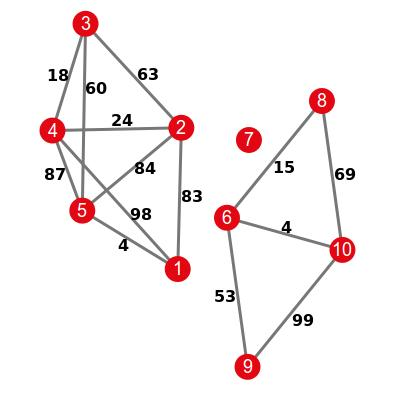
\includegraphics[scale=0.5]{imagenes/ejemplopetroleo.jpeg}
\end{center}
  \caption{Ejemplo de pozos y posibles tuberías}\label{fig:ejpetroleo}
\endminipage
\minipage{0.5\textwidth}
\begin{center}
  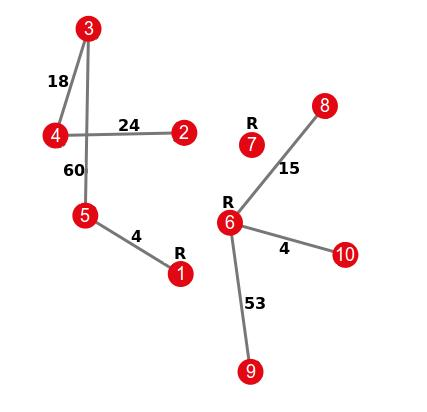
\includegraphics[scale=0.5]{imagenes/ejemplopetroleores.jpeg}
\end{center}
  \caption{Solución para el problema de la Figura \ref{fig:ejpetroleo}}\label{fig:ejpetroleores}
\endminipage
\end{figure}


\vspace*{0.6cm}

%\newpage
\subsection{Desarrollo de la idea y correctitud.}




%\vspace*{0.6cm}

%\newpage
\subsection{Análisis de complejidad.}

\vspace*{0.3cm}


\vspace*{0.6cm}

%\newpage
\subsection{Experimentación y gráficos.}

\vspace*{0.3cm}


\subsubsection{Test 1}

\vspace*{0.3cm}


\vspace*{0.6cm}

%\newpage
\subsubsection{Test 2}

\vspace*{0.3cm}


\vspace*{0.6cm}

%\newpage
\subsubsection{Test 3}

\vspace*{0.3cm}

